\nofiles
\documentclass[dvipdfmx]{article}
\usepackage{authblk}
\usepackage{hyperref}
\hypersetup{
    colorlinks,
    citecolor=black,
    filecolor=black,
    linkcolor=black,
    urlcolor=black
}
\usepackage{pdfpages}
\includepdfset{pagecommand={\thispagestyle{plain}}}

\begin{document}
\pagestyle{plain}
%%%%%%%%%%%%%%%%%%%%%%%%%%%
% 表紙
%%%%%%%%%%%%%%%%%%%%%%%%%%%
\thispagestyle{empty}
\noindent

\rule{\textwidth}{1pt}
\vspace{2pt}
\begin{flushright}
 \Huge
\begin{tabular}{@{}l}
Core Challenge 2022\\
Solver and Graph Descriptions\\[6pt]
{\Large Version 0.1}
\end{tabular}
\end{flushright}
\vspace{2pt}
\rule{\textwidth}{1pt}
\vspace{10em}


\centering
{\Large Edited by}\\[2em]

{\huge Takehide Soh}\\[0.5em]
{\Large Kobe University, Japan}\\[2em]
{\huge Yoshio Okamoto}\\[0.5em]
{\Large The University of Electro-Communications, Japan}\\[2em]
{\huge Takehiro Ito}\\[0.5em]
{\Large Tohoku University, Japan}\\


%%%%%%%%%%%%%%%%%%%%%%%%%%%
% Table of contents
%%%%%%%%%%%%%%%%%%%%%%%%%%%
\newpage
\begin{flushleft}
    \tableofcontents
\end{flushleft}

%%%%%%%%%%%%%%%%%%%%%%%%%%%
% Solver Contents
%%%%%%%%%%%%%%%%%%%%%%%%%%%
\newpage
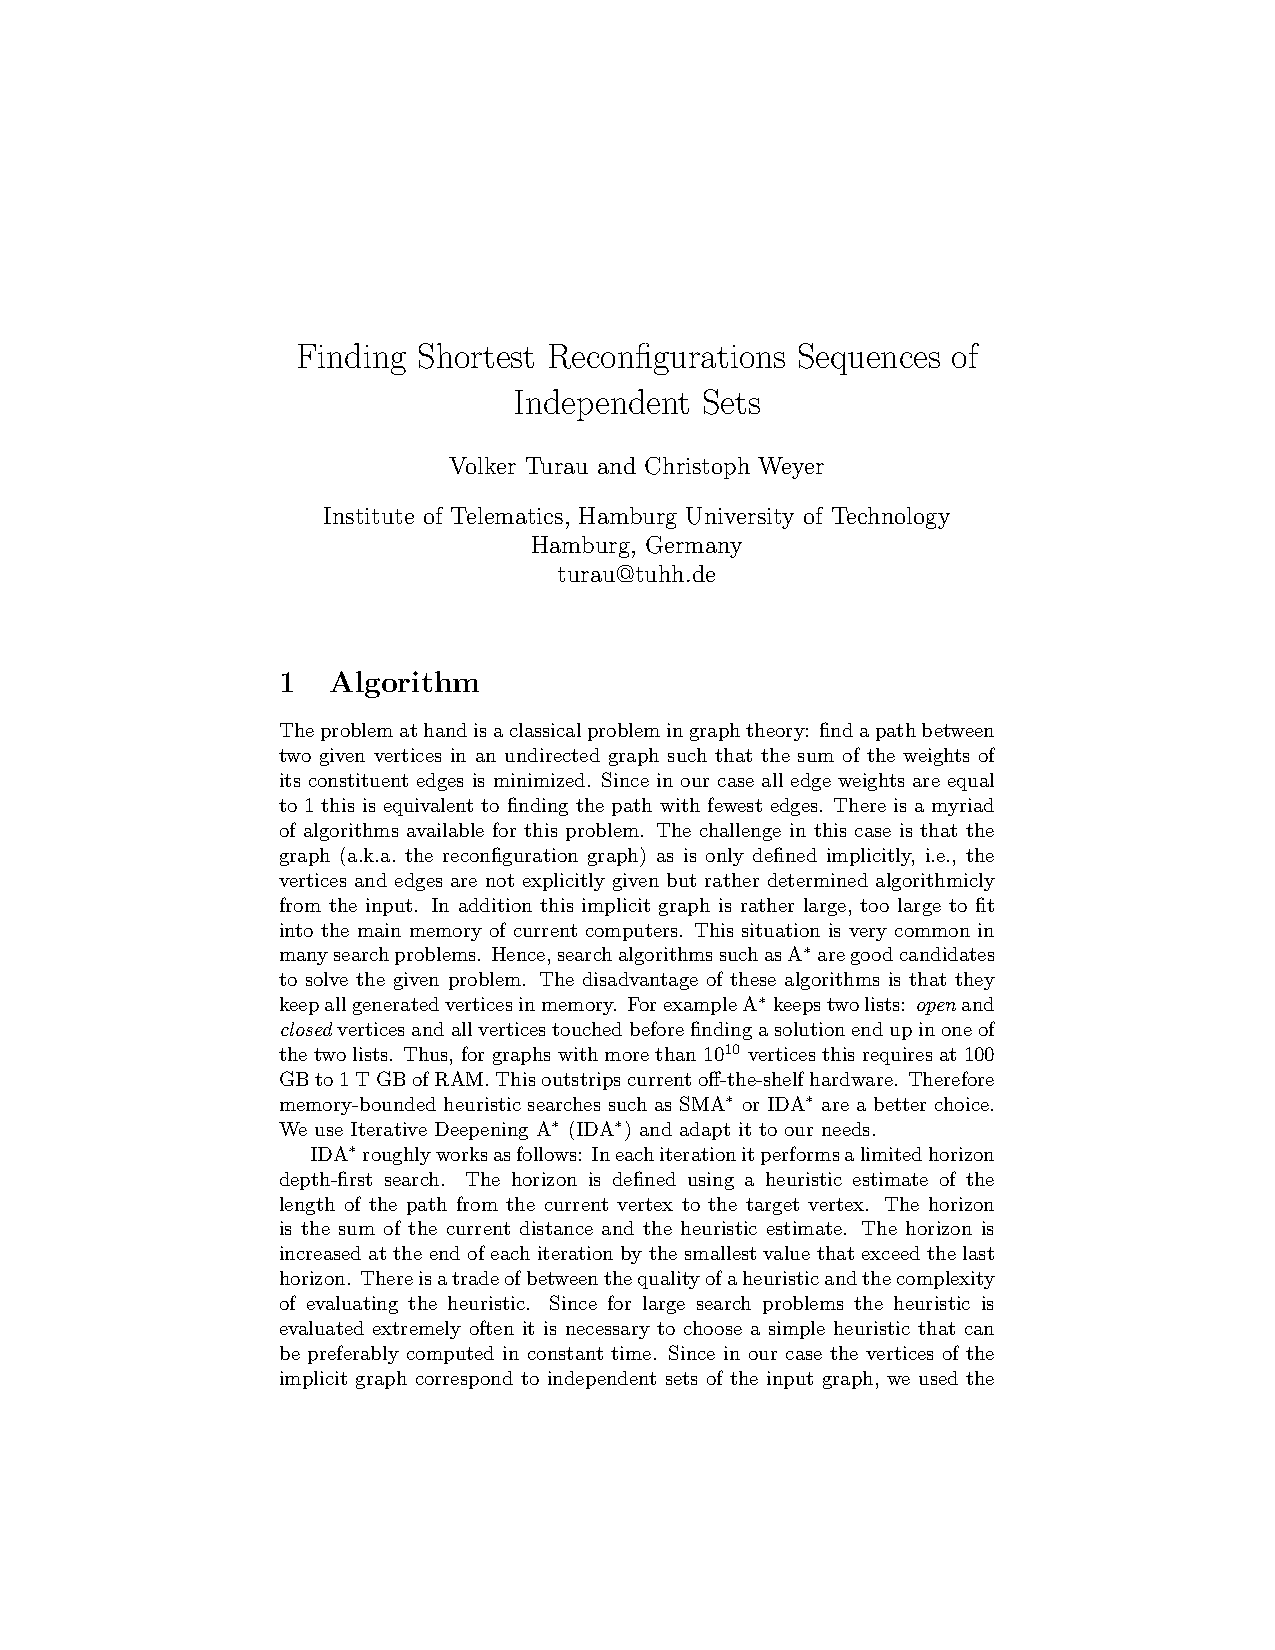
\includepdf[pages=-, addtotoc={1, section, 1, Finding Shortest Reconfigurations Sequences of Independent Sets, lbl:sub03-sol}]{submission03/solver/doc/solver.pdf}

\newpage
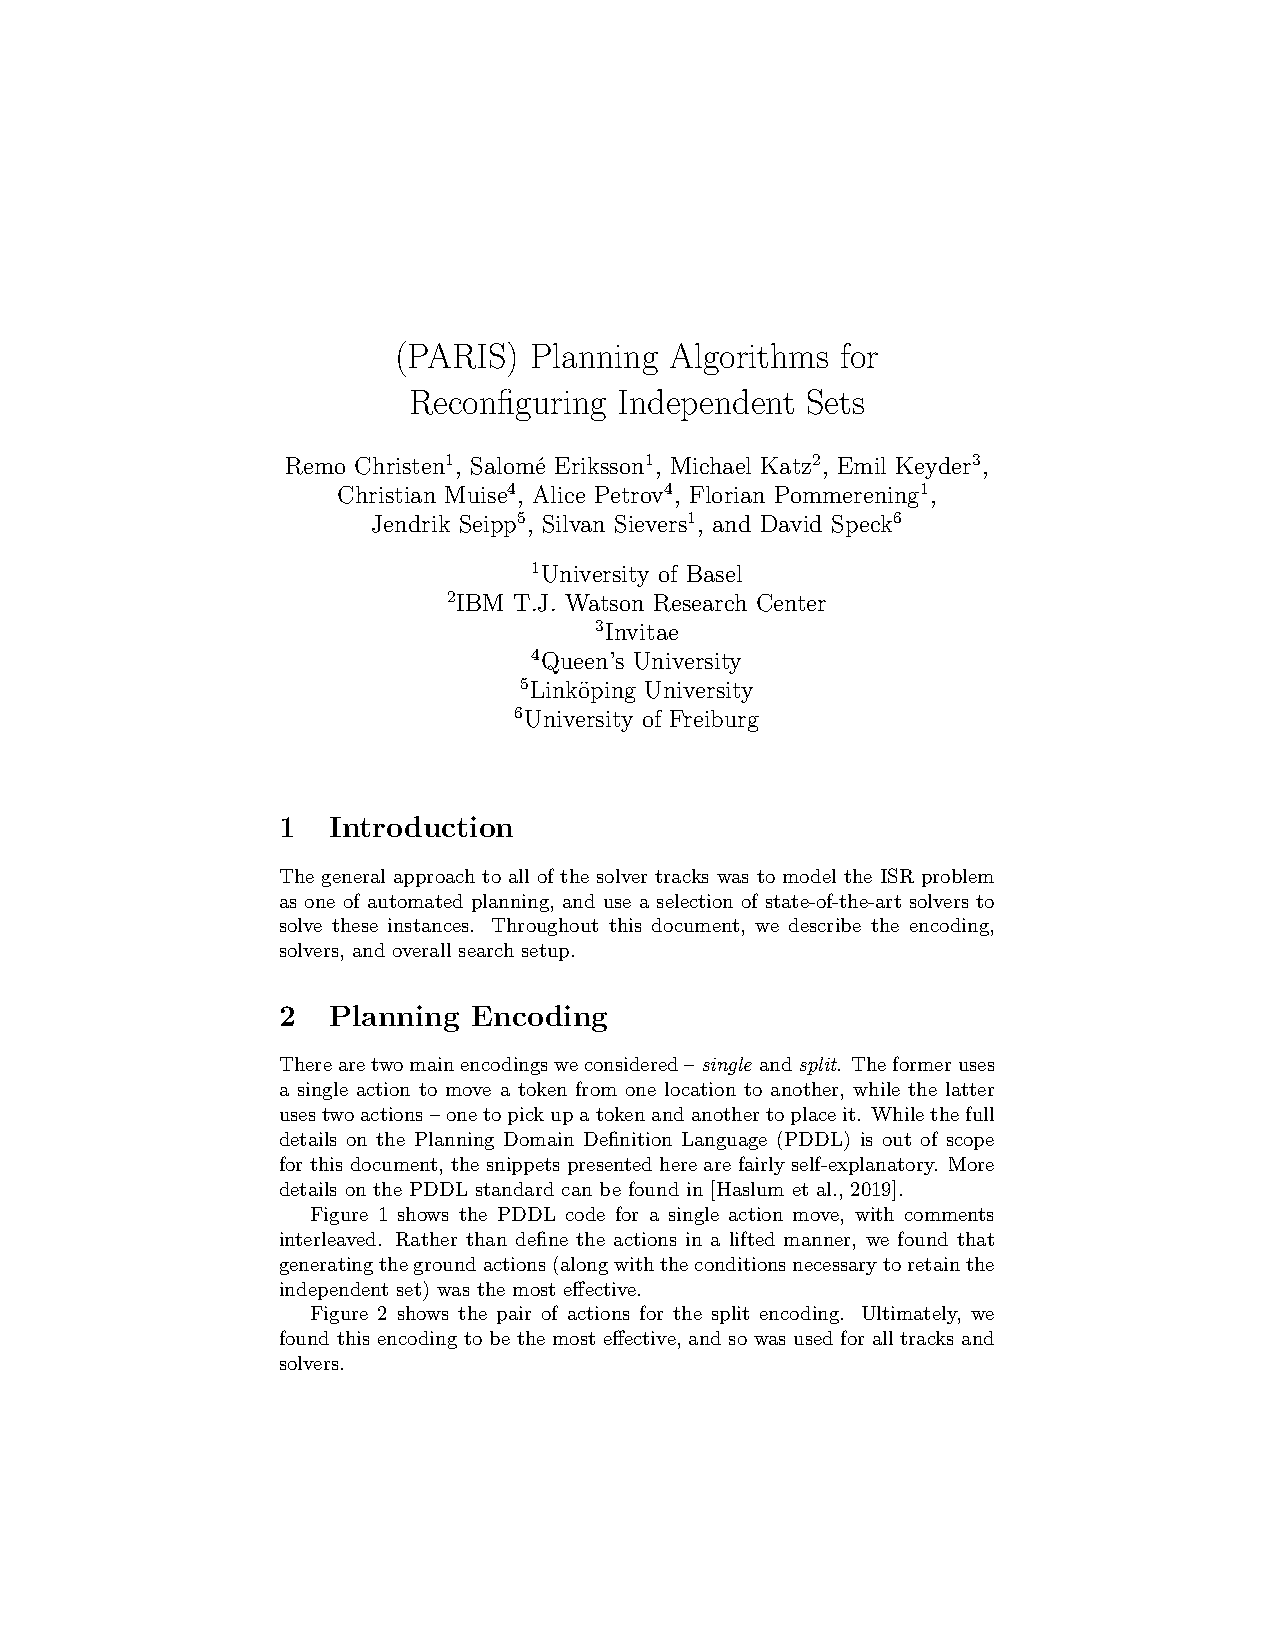
\includepdf[pages=-, addtotoc={1, section, 1, (PARIS) Planning Algorithms for Reconfiguring Independent Sets, lbl:sub04-sol}]{submission04/solver/doc/ISR_Solver_Track_Document.pdf}

\newpage
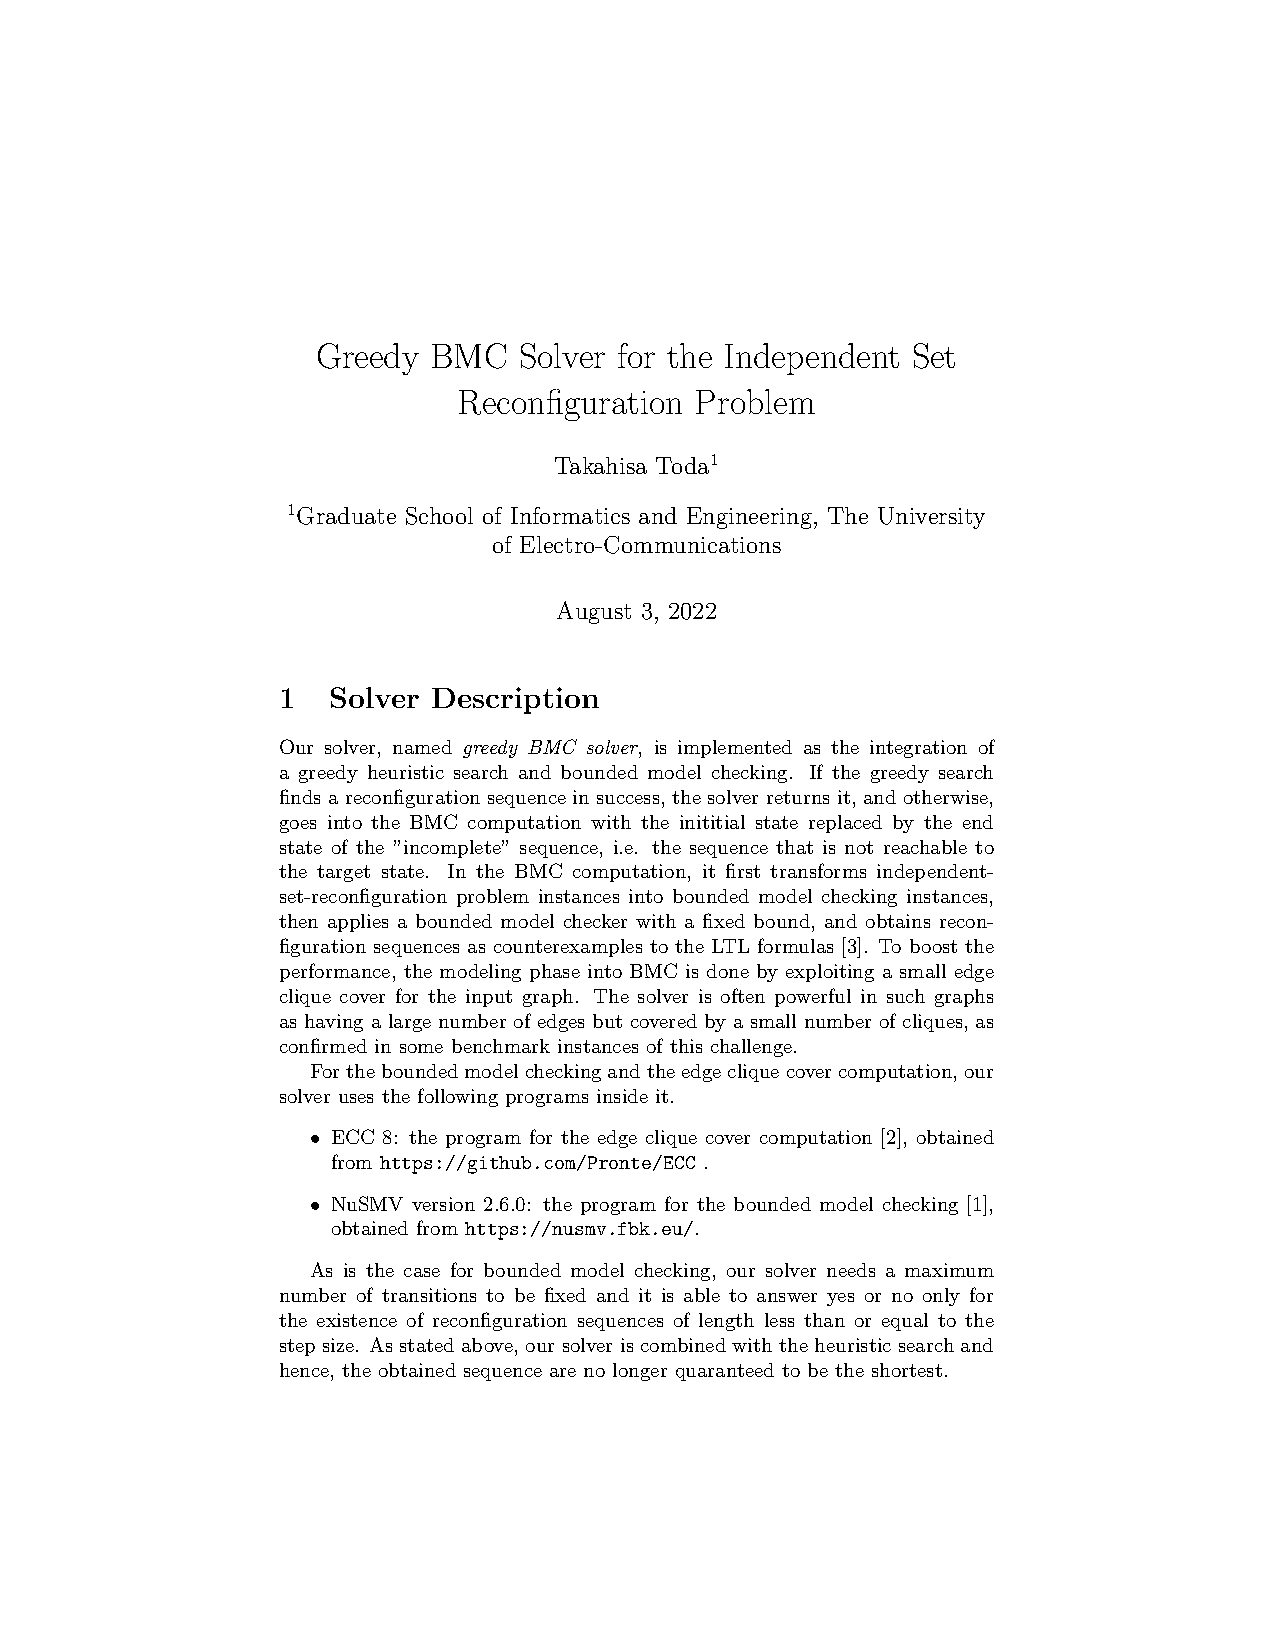
\includepdf[pages=-, addtotoc={1, section, 1, Greedy BMC Solver for the Independent Set Reconfiguration Problem, lbl:sub05-sol}]{submission05/solver/doc/example.pdf}

\newpage
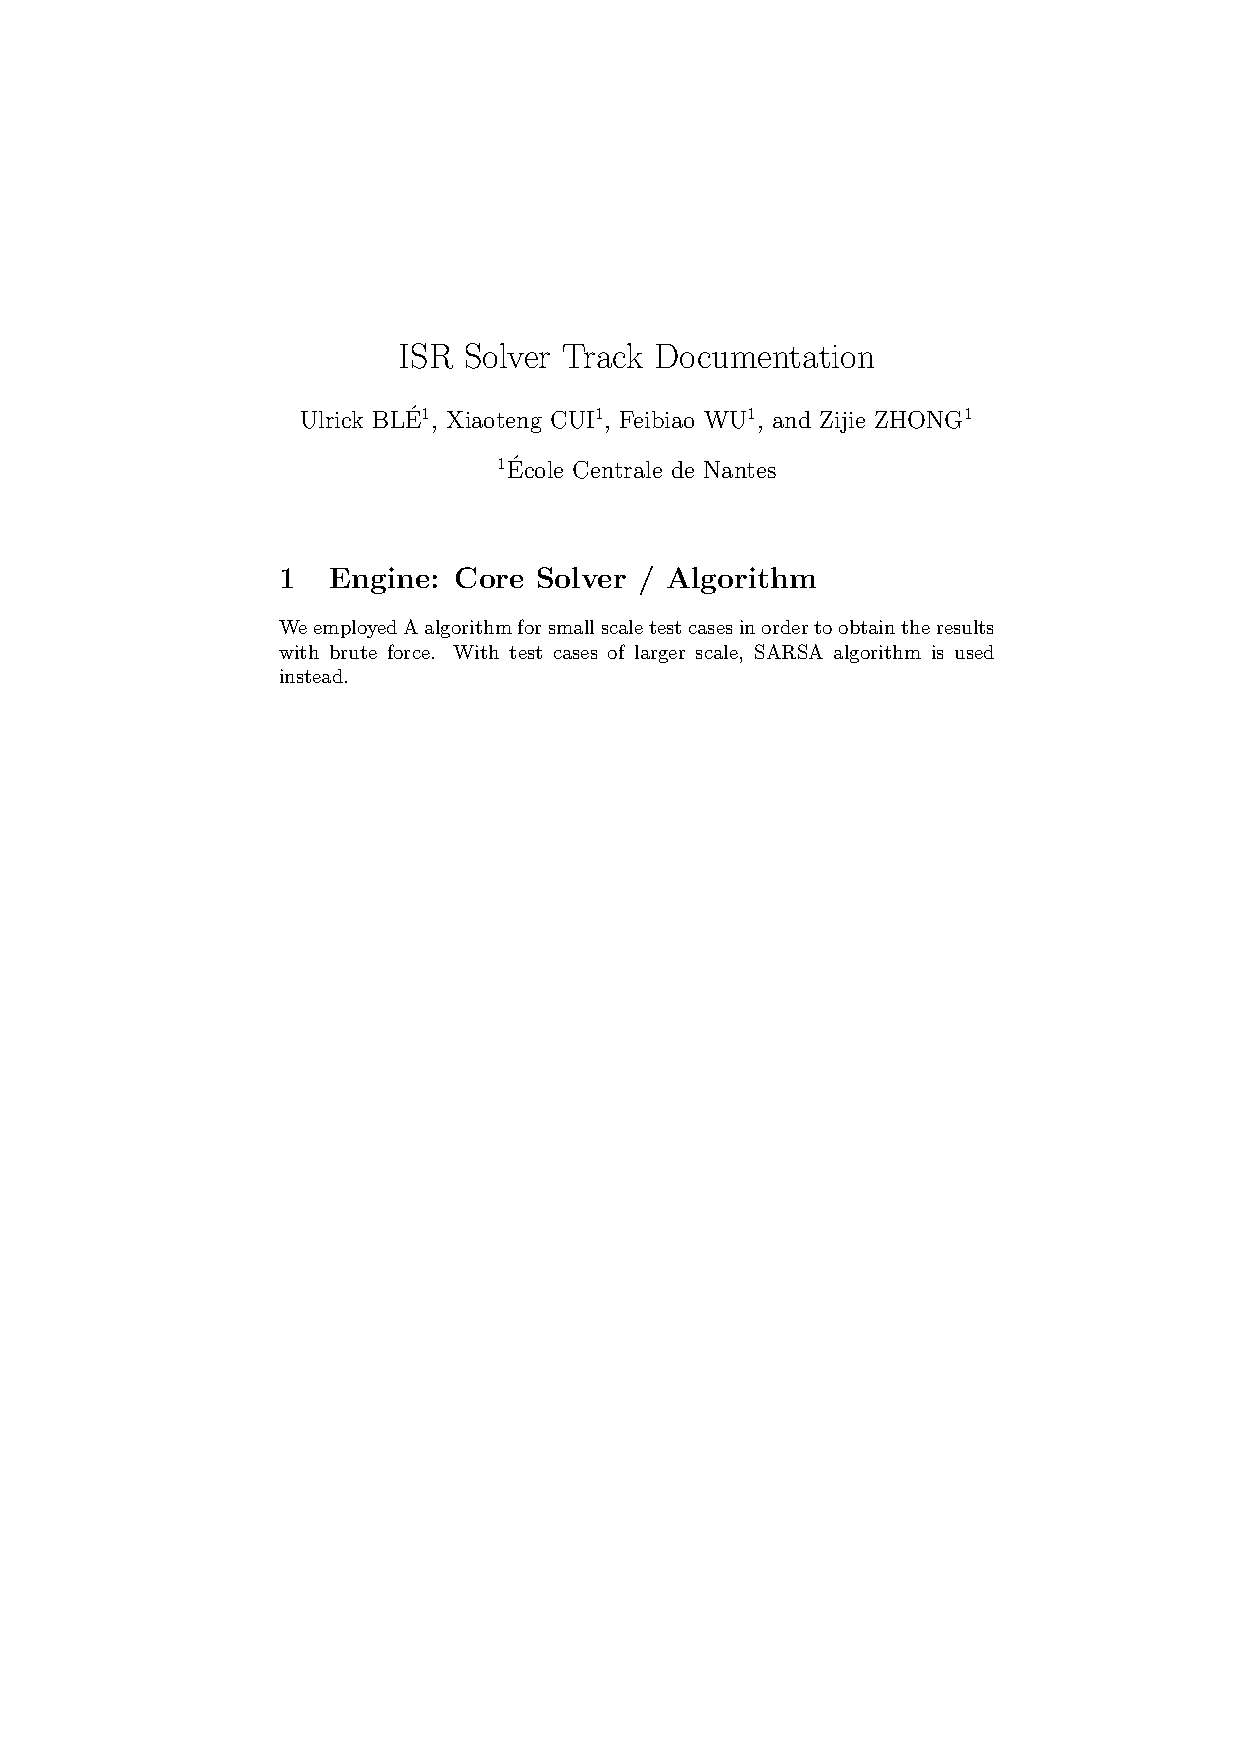
\includepdf[pages=-, addtotoc={1, section, 1, ISR Solver Track Documentation, lbl:sub06-sol}]{submission06/solver/doc/solver_track.pdf}

\newpage
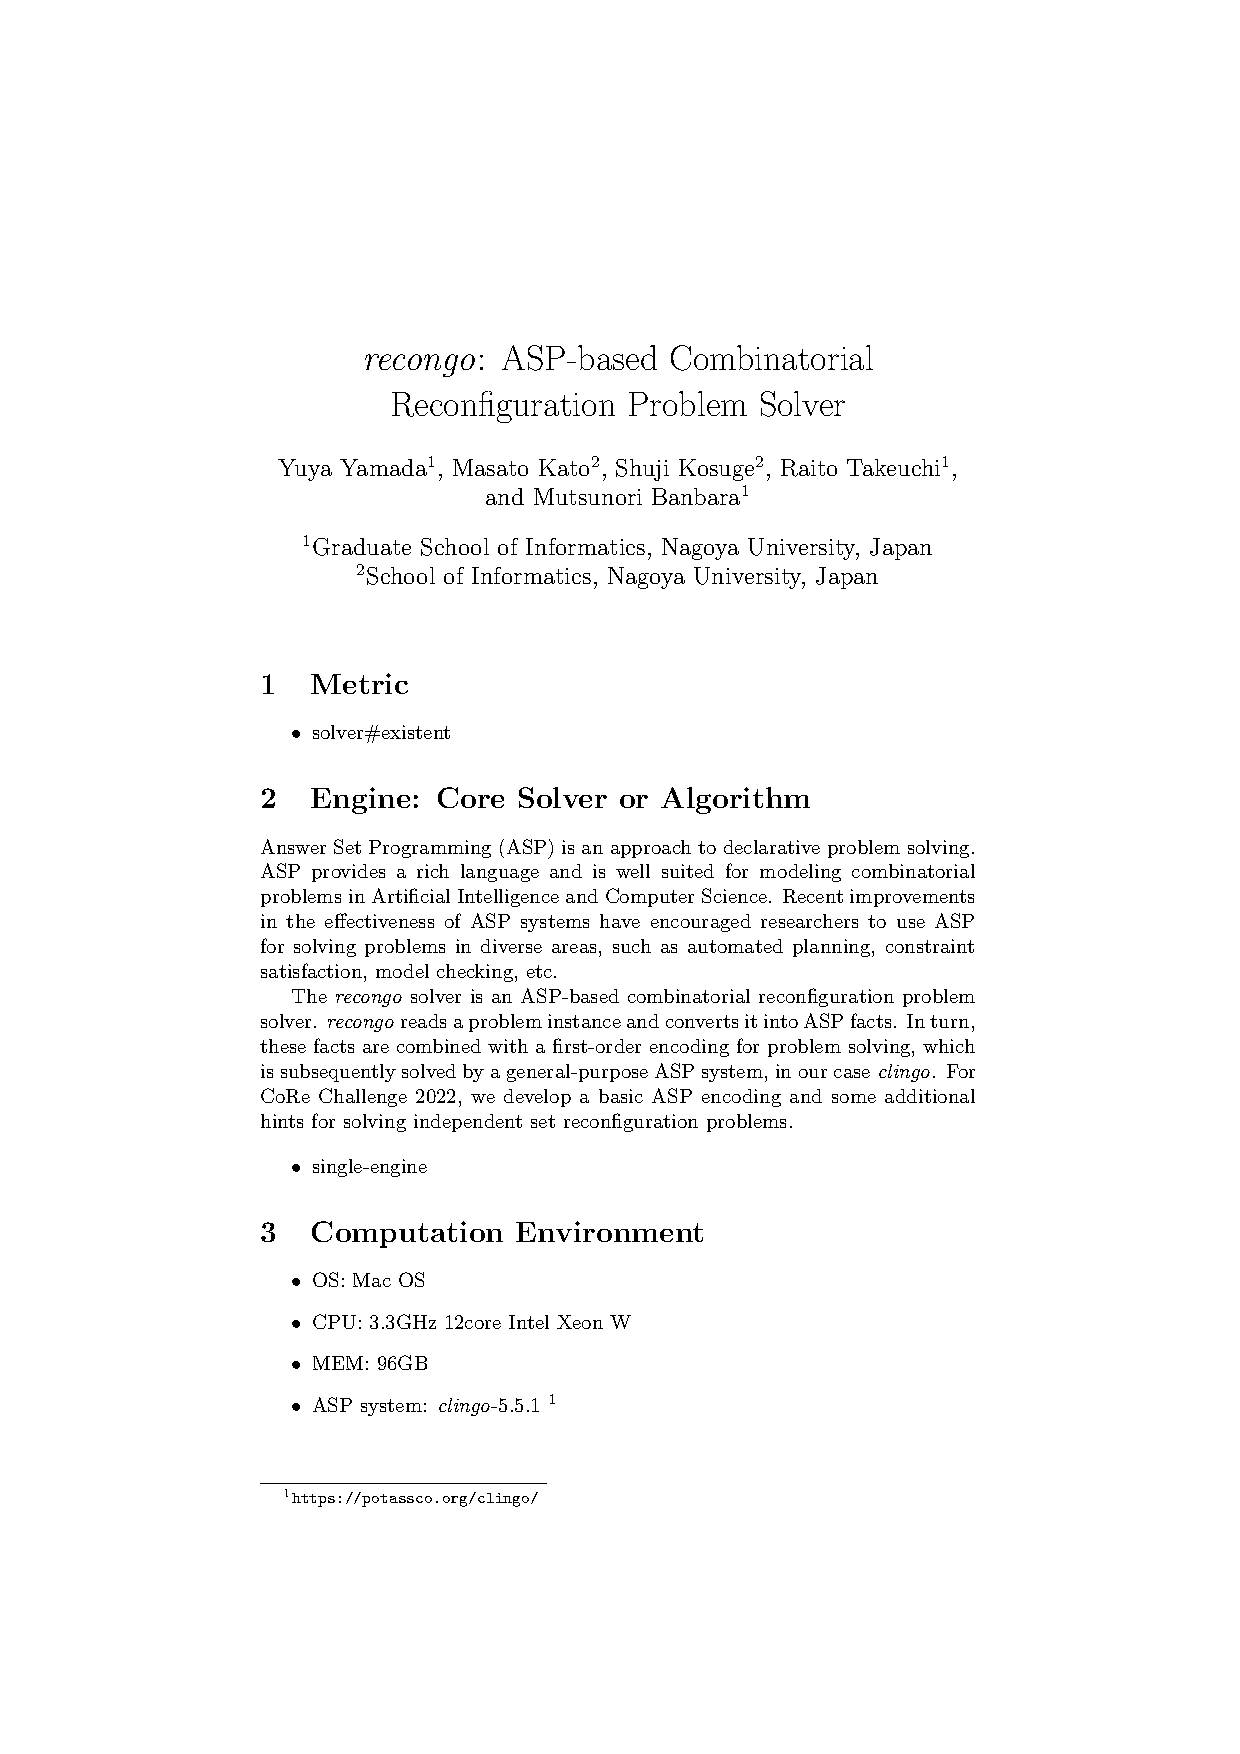
\includepdf[pages=-, addtotoc={1, section, 1, recongo: ASP-based Combinatorial Reconfiguration Problem Solver, lbl:sub07-sol}]{submission07/description/paper.pdf}

\newpage
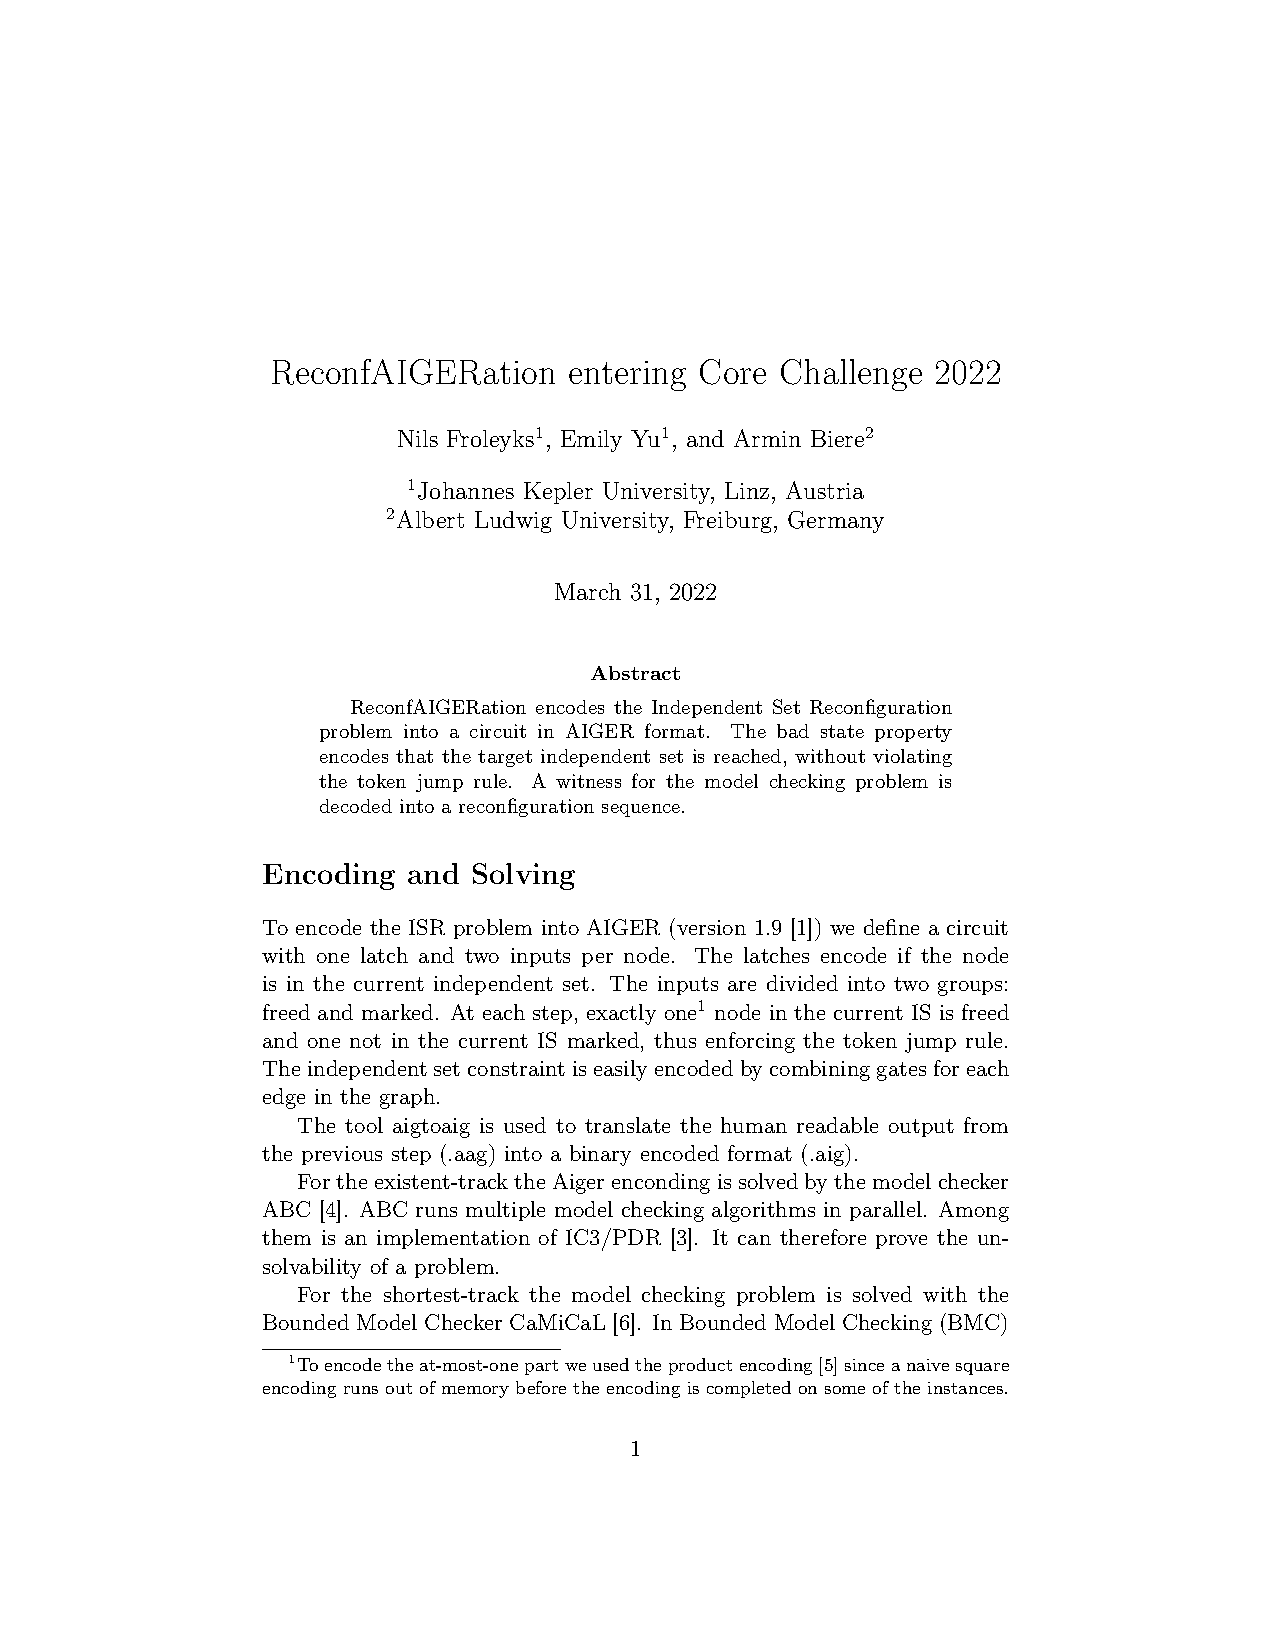
\includepdf[pages=-, addtotoc={1, section, 1, ReconfAIGERation entering Core Challenge 2022, lbl:sub011-sol}]{submission11/doc/reconfaigeration.pdf}

\newpage
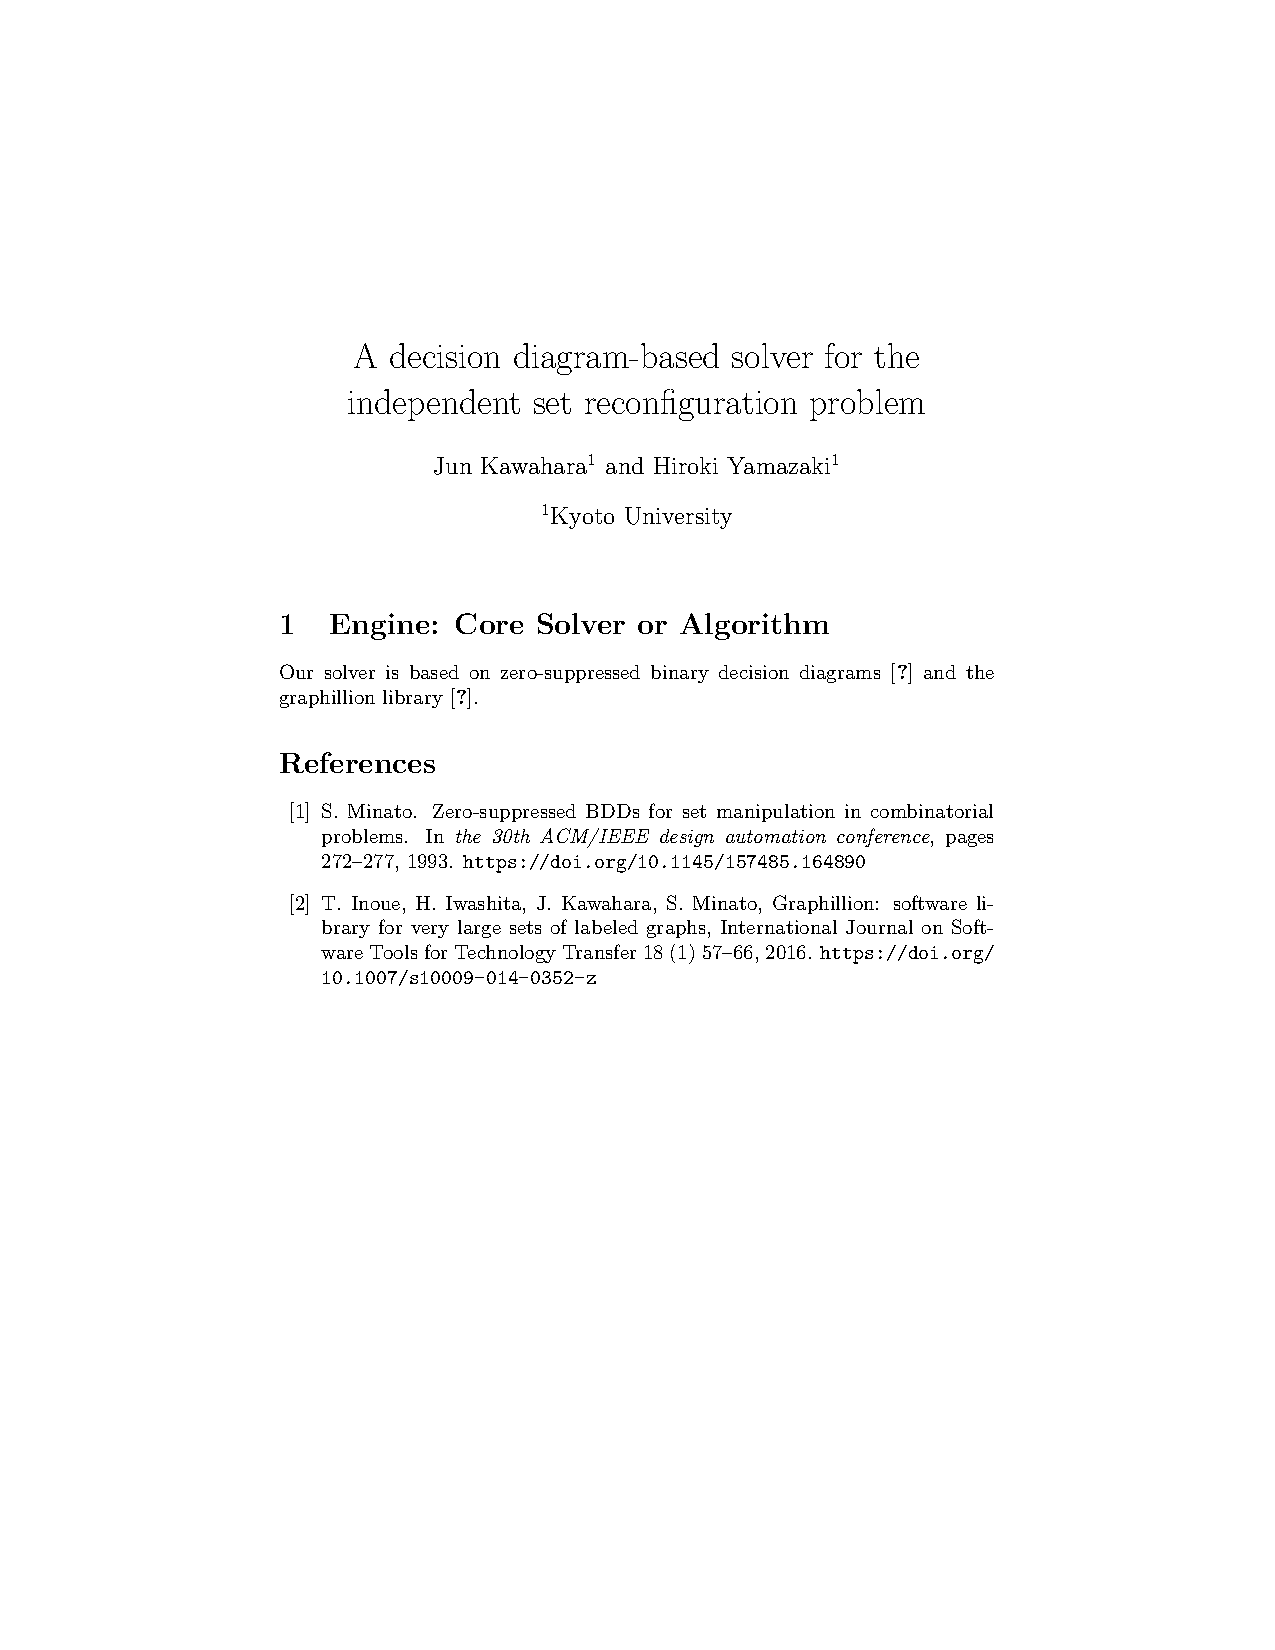
\includepdf[pages=-, addtotoc={1, section, 1, A decision diagram-based solver for the independent set reconfiguration problem, lbl:sub12-sol}]{submission12/description_zdd-solver.pdf}

%%%%%%%%%%%%%%%%%%%%%%%%%%%
% Graph Contents
%%%%%%%%%%%%%%%%%%%%%%%%%%%
\newpage
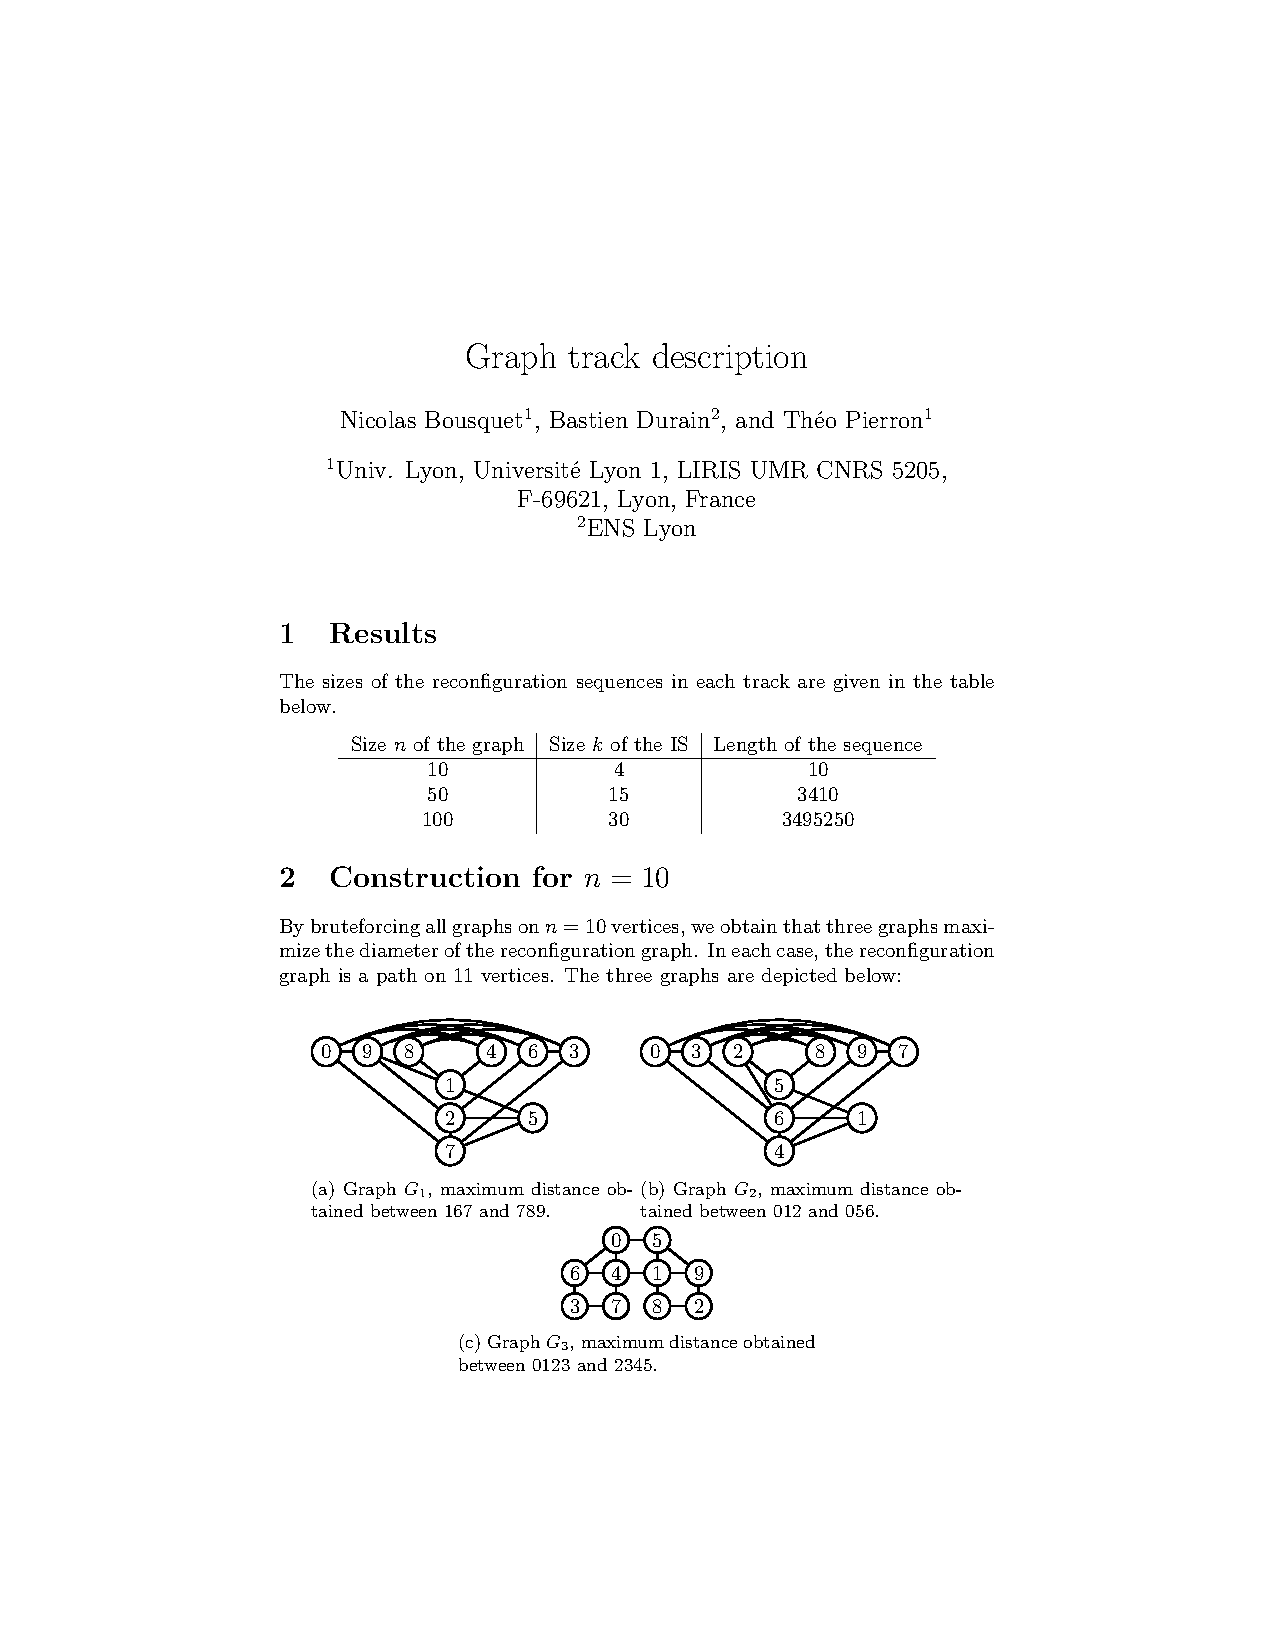
\includepdf[pages=-, addtotoc={1, section, 1, Graph track description, lbl:sub01-gra}]{submission01/graph/doc/example.pdf}

\newpage
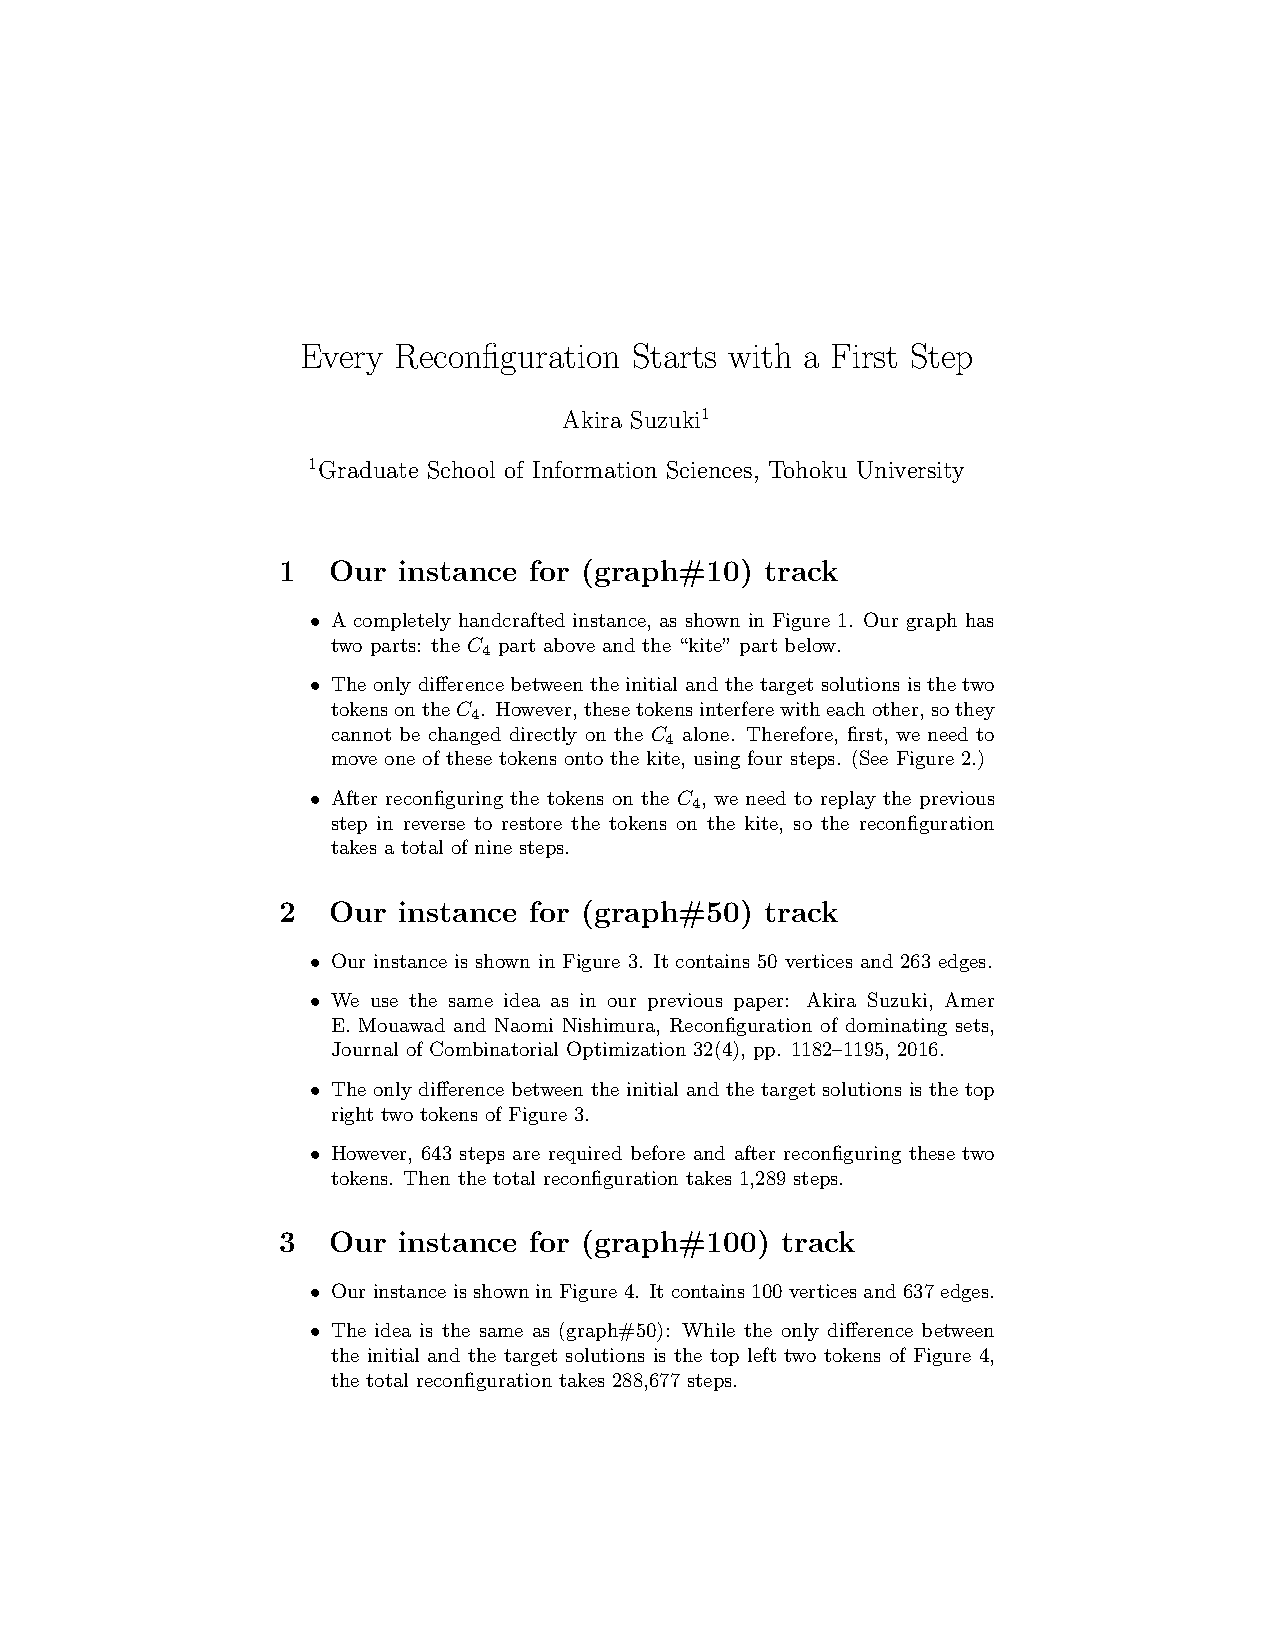
\includepdf[pages=-, addtotoc={1, section, 1, Every Reconfiguration Starts with a First Step, lbl:sub02-gra}]{submission02/doc/main.pdf}

\newpage
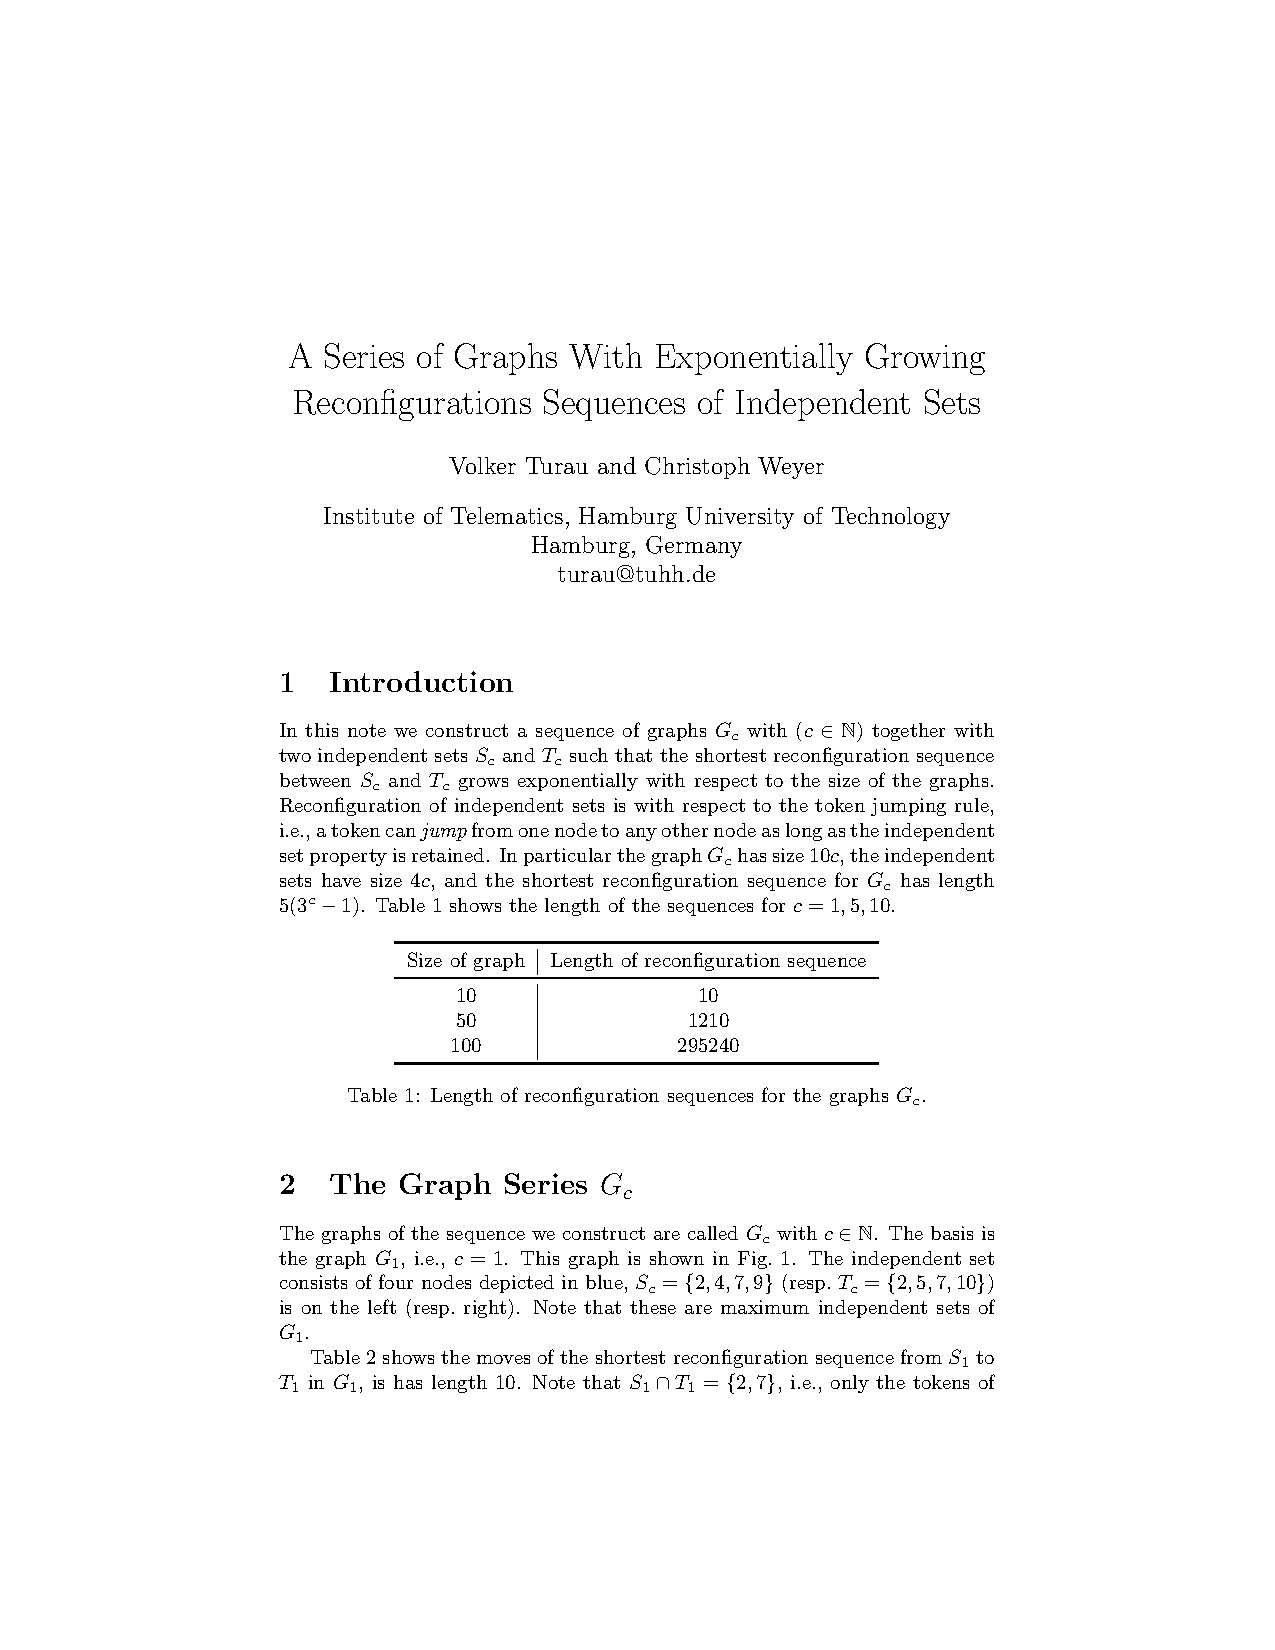
\includepdf[pages=-, addtotoc={1, section, 1, A Series of Graphs With Exponentially Growing Reconfigurations Sequences of Independent Sets, lbl:sub03-gra}]{submission03/graph/doc/submission.pdf}

\newpage
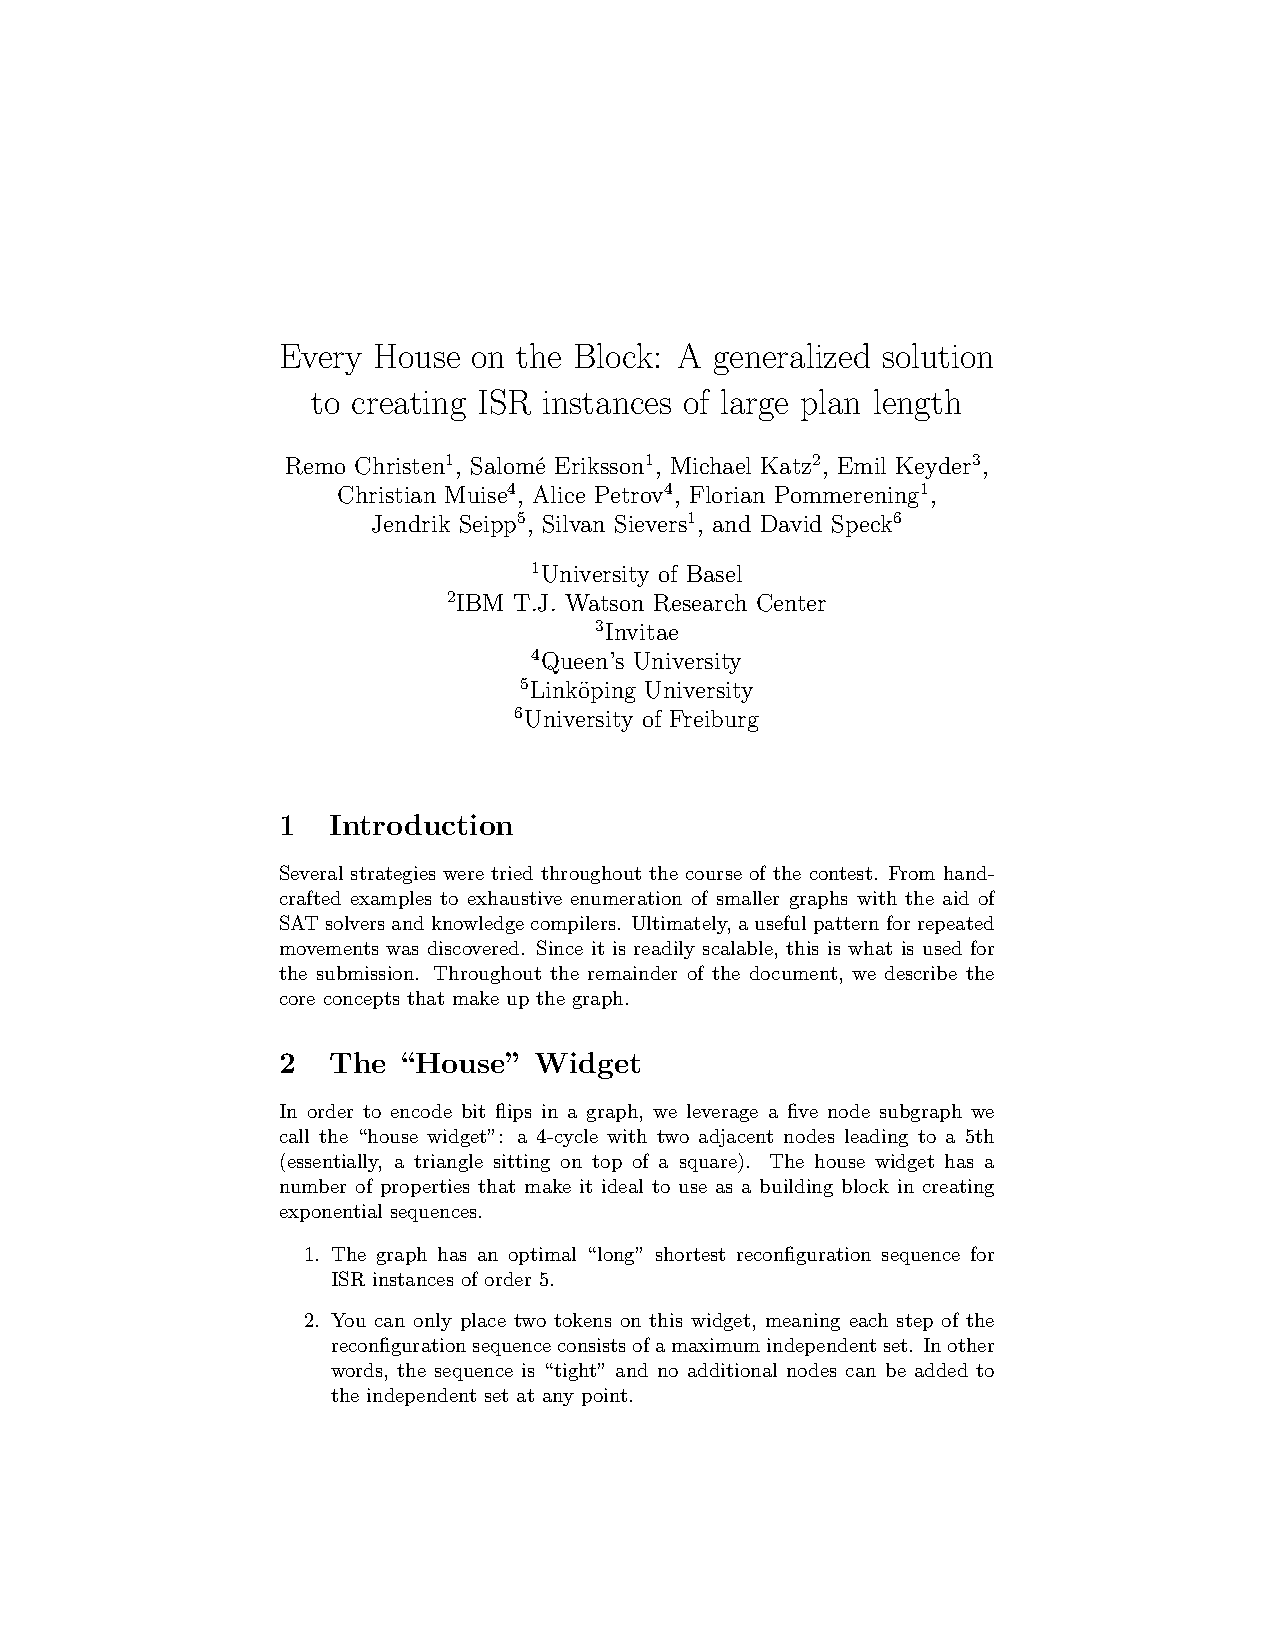
\includepdf[pages=-, addtotoc={1, section, 1, Every House on the Block: A generalized solution to creating ISR instances of large plan length, lbl:sub04-gra}]{submission04/graph/doc/ISR_Graph_Track_Documentation.pdf}

\newpage
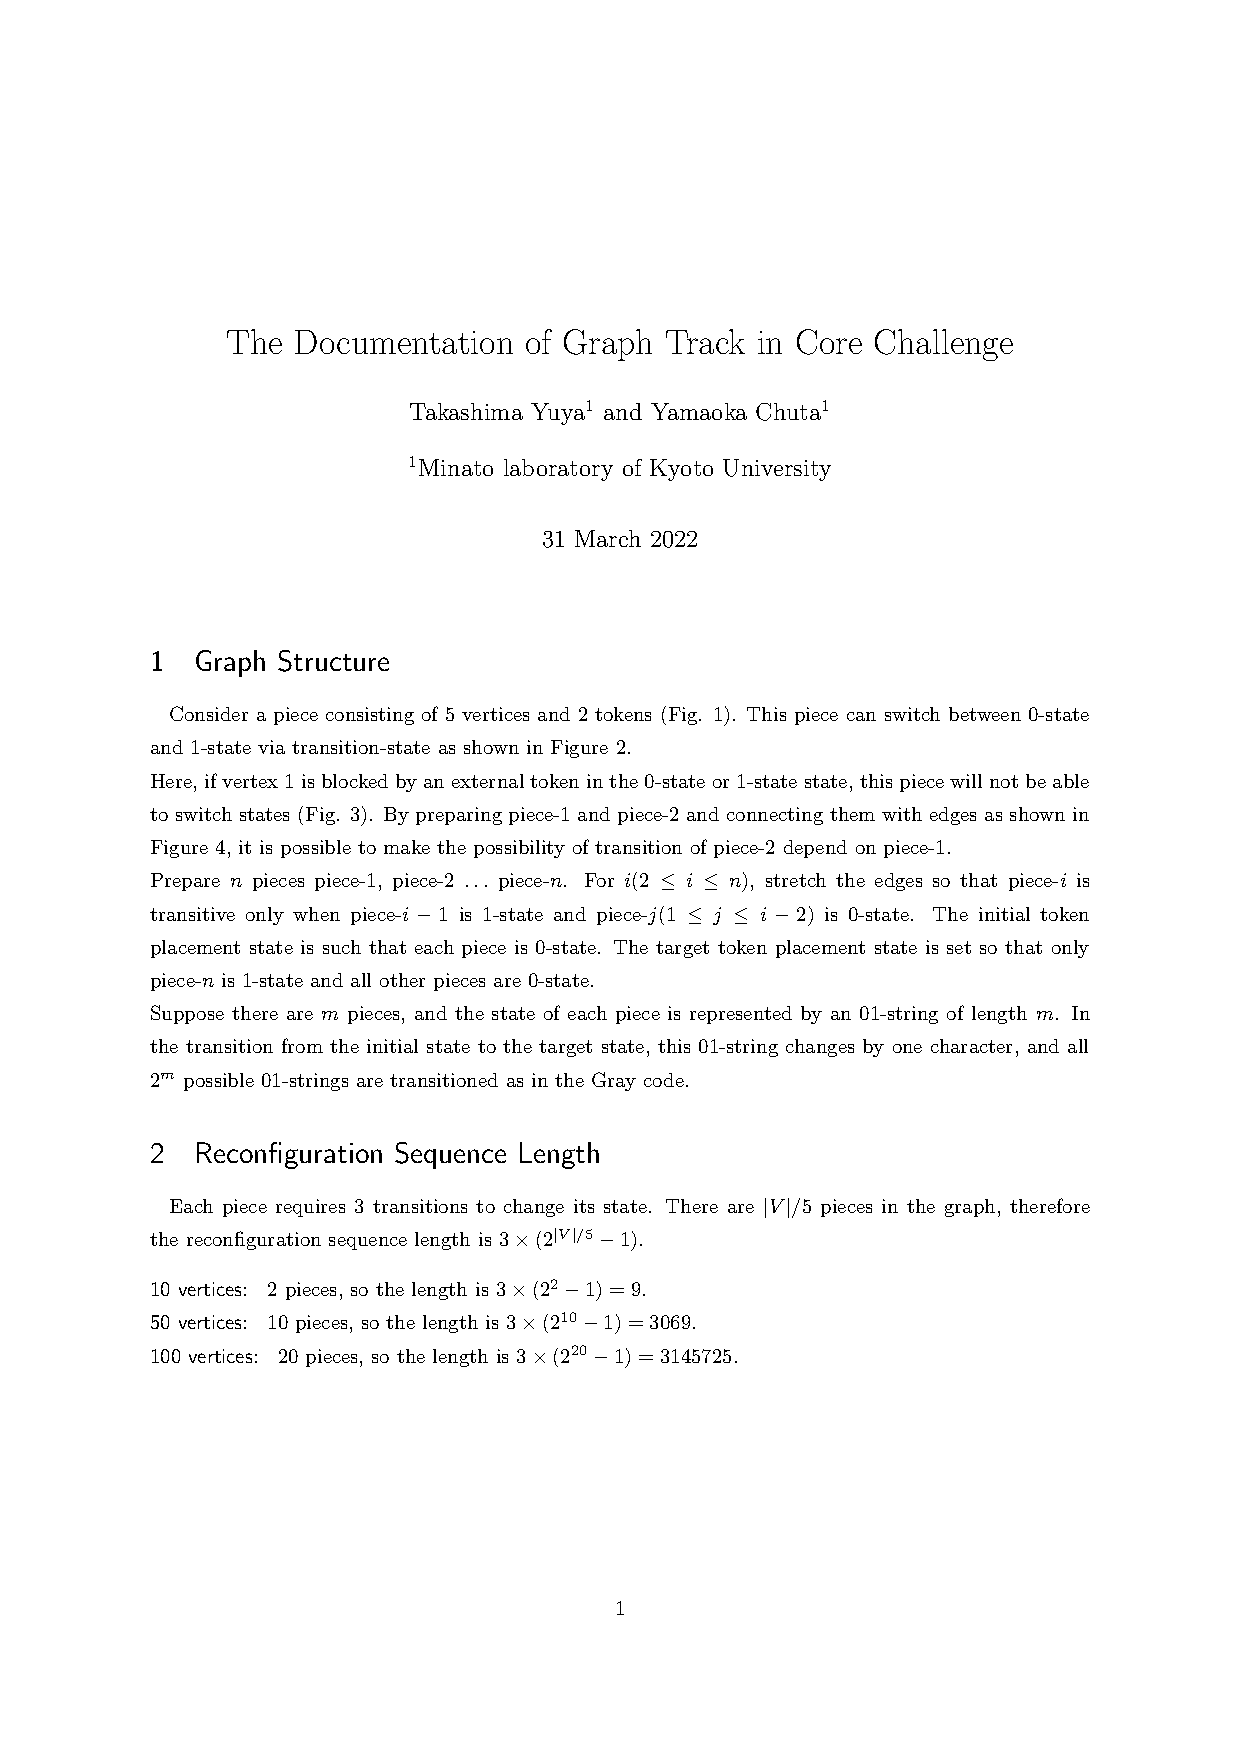
\includepdf[pages=-, addtotoc={1, section, 1, The Documentation of Graph Track in Core Challenge, lbl:sub10-gra}]{submission10/graph/doc/graph_track.pdf}


\end{document}
